% THIS IS SIGPROC-SP.TEX - VERSION 3.1
% WORKS WITH V3.2SP OF ACM_PROC_ARTICLE-SP.CLS
% APRIL 2009
%
% It is an example file showing how to use the 'acm_proc_article-sp.cls' V3.2SP
% LaTeX2e document class file for Conference Proceedings submissions.
% ----------------------------------------------------------------------------------------------------------------
% This .tex file (and associated .cls V3.2SP) *DOES NOT* produce:
%       1) The Permission Statement
%       2) The Conference (location) Info information
%       3) The Copyright Line with ACM data
%       4) Page numbering
% ---------------------------------------------------------------------------------------------------------------
% It is an example which *does* use the .bib file (from which the .bbl file
% is produced).
% REMEMBER HOWEVER: After having produced the .bbl file,
% and prior to final submission,
% you need to 'insert'  your .bbl file into your source .tex file so as to provide
% ONE 'self-contained' source file.
%
% Questions regarding SIGS should be sent to
% Adrienne Griscti ---> griscti@acm.org
%
% Questions/suggestions regarding the guidelines, .tex and .cls files, etc. to
% Gerald Murray ---> murray@hq.acm.org
%
% For tracking purposes - this is V3.1SP - APRIL 2009

\documentclass{acm_proc_article-sp}
\usepackage{float}

\begin{document}

\raggedbottom

\title{Distributed Histogram Creation with MapReduce and MPI}
\subtitle{CSC 569}

\numberofauthors{4} 
\author{
\alignauthor
Ian Dunn\\
       \affaddr{Computer Science Department}\\
       \affaddr{Cal Poly}\\
       \affaddr{San Luis Obispo, California}\\
       \email{idunn01@calpoly.edu}
\alignauthor
Toshi Kuboi\\
       \affaddr{Computer Science Department}\\
       \affaddr{Cal Poly}\\
       \affaddr{San Luis Obispo, California}\\
       \email{tkuboi@calpoly.edu}
       \and % go to new row
\alignauthor
Mitchell Rosen\\
       \affaddr{Computer Science Department}\\
       \affaddr{Cal Poly}\\
       \affaddr{San Luis Obispo, California}\\
       \email{mwrosen@calpoly.edu}
\alignauthor
Austin Wylie\\
       \affaddr{Computer Science Department}\\
       \affaddr{Cal Poly}\\
       \affaddr{San Luis Obispo, California}\\
       \email{awylie@calpoly.edu}
}

\date{30 October 2013}

\maketitle

\section{Introduction}
This project familiarized us with MapReduce, MPI, and distributed computing performance tradeoffs by calculating vector sums and histograms on a cluster of five Raspberry Pis. We wrote two programs that, given a pair of input files containing vectors of floating-point numbers, summed those vectors and created histograms for each of them as well as the vector sum.

One program's aim was to distribute the work among the five Pis and compute the results as quickly as possible. The other program made this process fault-tolerant (albeit less efficient) with a different method that allowed one node to be disconnected during its run.

\section{Part A: Distributed Performance}
This section describes our non-fault-tolerant program that distributes histogram creation among the five nodes.

\subsection{Program Setup}
Using MPI, this first program sends the input vector files residing on the master to the other four nodes as character arrays. Each node then breaks the input vector character arrays into large chunks and maps them.

The map callback tokenizes each large string on whitespace, converts each token into a float, and creates KeyValues with the float's index as the key and the float as the value. The addition happens after the two vector's MapReduce objects are combined (with MaprReduce's add and collate functions), and the results are reduced by summing the values for each index and creating new KeyValues with the index as key and the summed result as value.

Now that each of the three vectors (the third being the summed vector) are available, each one's maximum is found by performing a built-in MapReduce sort on the values and returning the first element of the vector.

Next, histogram counts are calculated with a map function that creates KeyValues with a bin number as key, a collate that combines them, and a reduce that counts the number of (empty or null) values per bin number. Those counts are then scanned into arrays on the master node, and are written to result files (in addition to the summed vector).

\subsection{Performance Analysis}
Performance analysis information.

\begin{table}[tbp]
\centering
\caption{Histogram Creation Performance}
\label{PiTable}
\begin{tabular}{ c || c }
	Input Size & Time \\ \hline
    10 & Time \\
    10,000 & Time \\
    100,000 & Time \\
    1,000,000 & Time \\
    10,000,000 & Time \\
\end{tabular}
\end{table}

\begin{figure}[tbp]
  \centering
  \caption{Histogram for 10-Count Vectors}
	\label{hist10}
  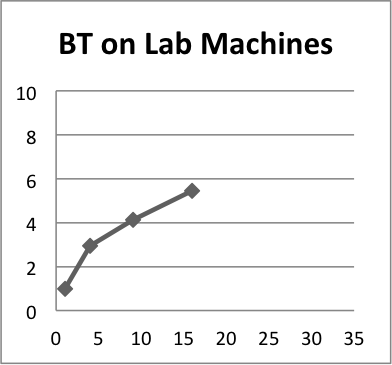
\includegraphics[width=19pc]{Pics/BT.png}
\end{figure}

\begin{figure}[tbp]
  \centering
  \caption{Histogram for 10,000-Count Vectors}
	\label{hist10000}
  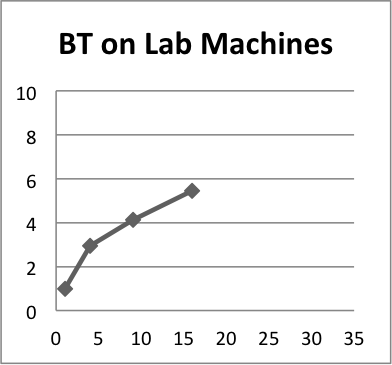
\includegraphics[width=19pc]{Pics/BT.png}
\end{figure}

\begin{figure}[tbp]
  \centering
  \caption{Histogram for 100,000-Count Vectors}
	\label{hist100000}
  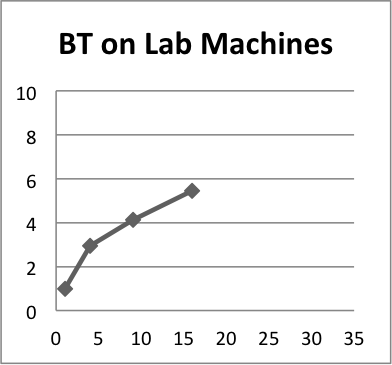
\includegraphics[width=19pc]{Pics/BT.png}
\end{figure}

\begin{figure}[tbp]
  \centering
  \caption{Histogram for 1,000,000-Count Vectors}
	\label{hist1000000}
  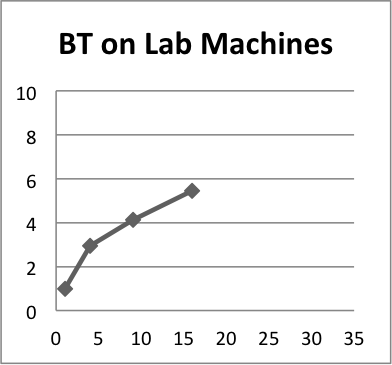
\includegraphics[width=19pc]{Pics/BT.png}
\end{figure}

\begin{figure}[tbp]
  \centering
  \caption{Histogram for 10,000,000-Count Vectors}
	\label{hist10000000}
  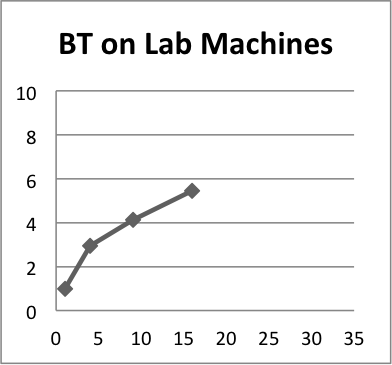
\includegraphics[width=19pc]{Pics/BT.png}
\end{figure}

\section{Part B: Fault-Tolerance}
This section describes our fault-tolerant program that distributes histogram creation among the five nodes.

\subsection{Program Setup}
Setup description.

\subsection{Performance Analysis}
Performance analysis information.


\bibliographystyle{abbrv}
%\bibliography{sample}

%\balancecolumns 

\end{document}
